% Comment lines start with %
% LaTeX commands start with \
% This template was provided by Jennifer Welch for CSCE 222-200, Honors, Spring 2015

\documentclass[12pt]{article}  % This is an article with font size 12-point

% Packages add features
\usepackage{times}     % font choice
\usepackage{amsmath}   % American Mathematical Association math formatting
\usepackage{amsthm}    % nice formatting of theorems
\usepackage{amssymb}    % provides some symbols
\usepackage{latexsym}  % provides some more symbols
\usepackage{fullpage}  % uses most of the page (1-inch margins)
\usepackage[shortlabels]{enumitem}
\usepackage{graphicx}

\setlength{\parskip}{.1in}  % increase the space between paragraphs

\renewcommand{\baselinestretch}{1.1}  % increase the space between lines

% Convenient renaming of symbols for logic formulas
\newcommand{\NOT}{\neg}
\newcommand{\AND}{\wedge}
\newcommand{\OR}{\vee}
\newcommand{\XOR}{\oplus}
\newcommand{\IMPLIES}{\rightarrow}
\newcommand{\IFF}{\leftrightarrow}
\providecommand{\myceil}[1]{$\left \lceil #1 \right \rceil$}
\providecommand{\myfloor}[1]{$\left \lfloor #1 \right \rfloor$}
\newcommand{\powerset}[1]{\mathbb{P}(#1)}

% Actual content starts here.
\begin{document}

\begin{center}         % center all the material between begin and end
{\large                % use larger font
CSCE 222 (Carlisle), Discrete Structures for Computing \\  % \\ is line break
Spring 2022 \\
Homework 12}
\end{center}
\rule{6in}{.1pt}       % horizontal line 6 inches long and .1 point high
\begin{center}
{\large
Type your name below the pledge to sign\\
On my honor, as an Aggie, I have neither given nor received unauthorized aid on this academic work.\\
HUY QUANG LAI}
\end{center}

% blank line separates paragraphs.  First line of a paragraph is automatically
% indented.  

\rule{6in}{.1pt}       % horizontal line 6 inches long and .1 point high
                    
\noindent              % don't indent
{\bf Instructions:}    % \bf makes text boldface
                       % \em makes text emphasized (italics)

\begin{itemize}        % makes an itemized list
\item The exercises are from the textbook.  You are encouraged to work
      extra problems to aid in your learning; remember, the solutions to 
      the odd-numbered problems are in the back of the book.
\item Grading will be based on correctness, clarity, and whether your
      solution is of the appropriate length.
\item Always justify your answers.
\item Don't forget to acknowledge all sources of assistance in the section below, and write up your solutions on your own.
\item {\em Turn in .pdf file to Gradescope by the start of class on Monday, April 25, 2022.}  It is simpler to put each problem on its own page using the LaTeX clearpage command.
\end{itemize}


\rule{6in}{.1pt}       % horizontal line 6 inches long and .1 point high

{\bf Help Received:}    % \bf makes text boldface
\begin{itemize}
\item Rosen, Kenneth H. \textit{Discrete Mathematics and Its Applications}. McGraw-Hill, 2019.
\end{itemize}



\rule{6in}{.1pt}       % horizontal line 6 inches long and .1 point high

%---------------------------------------------------------------------

% \subsection makes a subsection heading; * leaves it unnumbered.
% (Usually subsections are inside sections, but the \section command
% used a font that was larger than I wanted.)
\subsection*{Exercises for Section 9.1:}     

\noindent
{\bf 4(a-d): (2 points).}

\noindent
Determine whether the relation $R$ on the set of all people is reflexive, symmetric, antisymmetric, and/or transitive, where $(a,b)\in\mathbb{R}$ if and only if
\begin{enumerate}[a)]
    \item $a$ is taller than $b$\\
    Not reflexive: $a$ cannot be taller than $a$.\\
    Antisymmetric: If $a$ is taller than $b$, $b$ cannot be taller than $a$\\
    Not symmetric: $a$ is taller than $b$, $b$ cannot be taller than $a$\\
    Transitive: If $a$ is taller than $b$ and $b$ is taller than $c$, then $a$ must be taller than $c$.
    
    \item $a$ and $b$ were born on the same day.\\
    Reflexive: $a$ is born on $a$'s birthday.\\
    Symmetric: If $a$ was born on $b$’s birthday, then $b$ will be born on $a$’s birthday.\\
    Not antisymmetric: If $a$ was born on $b$'s birthday, then $b$ will be bor on $a$'s birthday.\\
    Transitive: If $a$ and $b$ share a birthday, and $b$ and $c$ share a birthday, then $a$ and $c$ must share a birthday.
    
    \item $a$ has the same first name as $b$.\\
    Reflexive: $a$ has the same first name as $a$\\
    Symmetric: If $a$ has the same first name as $b$, then $b$ has the same first name as $a$.\\
    Not antisymmetric: If $a$ has the same first name as $b$, then $b$ has the same first name as $a$.
    Transitive: If $a$ has the same first name as $b$ and $b$ has the same first name as $c$, then $a$ has the same first name as $c$
    
    \item $a$ and $b$ have a common grandparent.\\
    Reflexive: $a$ has a common grandparent with $a$.\\
    Symmetric: If $a$ has a common grandparent with $b$, then $b$ has a common grandparent with $a$.\\
    Not antisymmetric: If $a$ has a common grandparent with $b$, then $b$ has a common grandparent with $a$.\\
    Not Transitive: $a$ and $b$ can share a common grandparent $g$ while $b$ and $c$ can share a common grandparent $h$. However, $a$ and $c$ are not guaranteed to have a common grandparent.
\end{enumerate}

\clearpage
\noindent
{\bf 6(a,c,e,g): (2 points).}

\noindent
Determine whether the relation $R$ on the set of all real numbers is reflexive, symmetric, antisymmetric, and/or transitive, where $(x,y)\in\mathbb{R}$ if and only if
\begin{enumerate}[a)]
    \item $x+y=0$\\
    Not reflexive: $(1,1)\not\in R$\\
    Symmetric: $x+y=0=y+x$\\
    Not antisymmetric: $(-1,1)\land(1,-1)\in R$\\
    Not transitive: $(-1,1)\land(1,-1)\in R$ but $(1,1)\not\in R$
    
    \setcounter{enumi}{2}
    \item $x-y\in\mathbb{Q}$\\
    Reflexive: $x-x=0\in\mathbb{Q}$\\
    Symmetric: If $x-y\in\mathbb{Q}$, then $y-x=-(x-y)\in\mathbb{Q}$\\
    Not antisymmetric: If $x=1,y=2$ then $x-y\in\mathbb{Q}\land y-x\in\mathbb{Q}$ but $x\neq y$\\
    Transitive: If $x-y\in\mathbb{Q}\land y-z\in\mathbb{Q}$, then $x-z=(x-y)+(y-z)\in\mathbb{Q}$
    
    \setcounter{enumi}{4}
    \item $xy\geq0$\\
    Reflexive: $x^2\geq0$\\
    Symmetric: $xy=yx\geq0$\\
    Not antisymmetric: If $x=1,y=2$, then $xy\geq0\land yx\geq0$ but $x\neq y$\\
    Not transitive: If $x=1,y=0,z=-1$, then $xy\geq 0\land yz\geq0$ but $xz<0$
    
    \setcounter{enumi}{6}
    \item $x=1$\\
    Not reflexive: $(2,2)\not\in R$\\
    Not symmetric: $(1,2)\in R$ but $(2,1)\not\in R$\\
    Antisymmetric: If $(x,y)$ and $(y,x)$ are in $R$, then $x=1=y$\\
    Transitive: If $(x,y)$ and $(y,z)$ are in $R$, then $x=1$ and $(x,z)=(1,z)$ which is in $R$.
\end{enumerate}

\clearpage
\noindent
{\bf 34(a,c,e,g): (2 points).}

\noindent
$R_1=\{(a,b)\in\mathbb{R}^2|a>b\}$\\
$R_2=\{(a,b)\in\mathbb{R}^2|a\geq b\}$\\
$R_3=\{(a,b)\in\mathbb{R}^2|a<b\}$\\
$R_4=\{(a,b)\in\mathbb{R}^2|a\leq b\}$\\
$R_5=\{(a,b)\in\mathbb{R}^2|a=b\}$\\
$R_6=\{(a,b)\in\mathbb{R}^2|a\neq b\}$

\noindent
Find
\begin{enumerate}[a)]
    \item $R_1\bigcup R_3$\\
    $R_6$
    \setcounter{enumi}{2}
    \item $R_2\bigcap R_4$\\
    $R_5$
    \setcounter{enumi}{4}
    \item $R_1-R_2$\\
    $\emptyset$
    \setcounter{enumi}{6}
    \item $R_1\oplus R_3$\\
    $R_6$
\end{enumerate}

\clearpage
\subsection*{Exercises for Section 9.5:}     

\noindent
{\bf 2(a,c,e): (2 points).}

\noindent
Which of these relations on the set of all people are equivalence relations? Determine the properties of an equivalence relation that the others lack.
\begin{enumerate}[a)]
    \item \{$(a,b)\vert a$ and $b$ are the same age\}\\
    This is a equivalence relation.
    \setcounter{enumi}{2}
    \item \{$(a,b)\vert a$ and $b$ share a common parent\}\\
    This is not an equivalence relation, since it is not transitive.\\
    $A$ is the child of $W$ and $X$, $B$ is the child of $X$ and $Y$, and $C$ is the child of $Y$ and $Z$.\\
    Then $A$ is related to $B$, and $B$ is related to $C$, but $A$ is not related to $C$.
    \setcounter{enumi}{4}
    \item \{$(a,b)\vert a$ and $b$ speak a common language\}\\
    This is not an equivalence relation, since it is not transitive.\\
    $A$ and $B$ both can speak English, $B$ and $C$ both can speak Chinese.\\
    However $A$ and $C$ cannot communicate.

\end{enumerate}

\noindent
{\bf 12: (2 points).}

\noindent
Show that the relation $R$ consisting of all pairs $(x,y)$ such that $x$ and $y$ are bit strings of length three or more that agree except perhaps in their first three bits is an equivalence relation on the set of all bit strings of length three or more.

\noindent
Suppose $A$ is the set of all bit strings of length three or more.\\
Define a relation $R$ on $A$ as $R=\{(x,y)\vert x$ and $y$ agree in their first three bits$\}$

\noindent
Reflexive since $x$ shares the first three bits with $x$. 

\noindent
Symmetric\\
Suppose $x,y\in A,(x,y)\in R$\\
If $x$ and $y$ agree in their first three bits, then $y$ and $x$ agree in their first three bits.

\noindent
Transitive\\
Suppose $x,y,z\in A,(x,y),(y,z)\in R$\\
If $x$ and $y$ agree in their first three bits and $y$ and $z$ agree in their first three bits, then $x$ and $z$ agree in their first three bits.

\noindent
Hence, $R$ is reflexive symmetric and transitive on $A$ and therefore, $R$ is an equivalence relation on $A$. 

\clearpage
\noindent
{\bf 16: (2 points).}

\noindent
Let $R$ be the relation on the set of ordered pairs of positive integers such that $((a,b),(c,d))\in\mathbb{R}$ if and only if $ad=bc$. Show that $R$ is an equivalence relation.

\noindent
Reflexive\\
Since $a\cdot b=b\cdot a$.\\
Then $((a,b),(a,b))\in R$

\noindent
Symmetric\\
Since $ad=bc\equiv bc=ab$\\
Then $((c,d),(a,b))\in R$

\noindent
Transitive\\
If $((a,b),(c,d)\in R\land((c,d),(e,f))\in R$\\
Then $ab=bc\land cf=de$

\noindent
{\bf 44(b,c,d): (2 points).}

\noindent
Which of these collections of subsets are partitions of the set of integers?
\begin{enumerate}[a)]
    \setcounter{enumi}{1}
    \item the set of positive integers and the set of negative integers\\
    This is not a partition, since $0$ is in neither set.
    
    \item the set of integers divisible by 3, the set of integers leaving a remainder of 1 when divided by 3, and the set of integers leaving a remainder of 2 when divided by 3.\\
    This is a partition by the division algorithm
    
    \item the set of integers less than $-100$, the set of integers with absolute value not exceeding $100$, and the set of integers greater than $100$\\
    This is a partition, since the second set mentioned is the set of all number between $-100$ and $100$, inclusive.
\end{enumerate}

\clearpage
\subsection*{Exercises for Section 9.6:}     

\noindent
{\bf 8(a-c): (2 points).}

\noindent
Determine whether the relations represented by these
zero–one matrices are partial orders.

\begin{enumerate}[a)]
    \item $\begin{bmatrix}
    1 & 0 & 1 \\
    1 & 1 & 0 \\
    0 & 0 & 1
    \end{bmatrix}$\\
    Reflexive because the matrix's diagonal is only $1$\\
    Antisymmetric because $m_{ij}=1\land m{ji}=1$ is only true when $i=j$.\\
    Not transitive $m_{21}=1\land m_{13}=1\land m_{23}=0$.\\
    Not a partial ordering since $R$ is not transitive.
    
    \item $\begin{bmatrix}
    1 & 0 & 0 \\
    0 & 1 & 0 \\
    1 & 0 & 1
    \end{bmatrix}$\\
    Reflexive because the matrix's diagonal is only $1$\\
    Antisymmetric because $m_{ij}=1\land m{ji}=1$ is only true when $i=j$.\\
    Transitive because $m{31}=1$ does not cause transitivity problems.\\
    $R$ is a partial ordering.
    
    \item $\begin{bmatrix}
    1 & 0 & 1 & 0 \\
    0 & 1 & 1 & 0 \\
    0 & 0 & 1 & 1 \\
    1 & 1 & 0 & 1
    \end{bmatrix}$\\
    Reflexive because the matrix's diagonal is only $1$\\
    Antisymmetric because $m_{ij}=1\land m{ji}=1$ is only true when $i=j$.\\
    Not transitive $m_{13}=1\land m_{34}=1\land m_{14}=0$.\\
    Not a partial ordering since $R$ is not transitive.
\end{enumerate}

\clearpage
\noindent
{\bf 34(a,c,f,h): (2 points).}

\noindent
Answer these questions for the poset $(\{2,4,6,9,12,18,27,36,48,60,72\},\vert)$.
\begin{enumerate}[a)]
    \item Find the maximal elements.\\
    $27$, $48$, $60$, and $72$ are maximal.\\
    Each divides no number in the list other than itself.\\
    All of the other numbers divide $72$ so they are not maximal
    
    \setcounter{enumi}{2}
    \item Is there a greatest element?
    There is no greatest element.\\
    There is no number in the set that both 60 and 72 divide
    
    \setcounter{enumi}{5}
    \item Find the least upper bound of $\{2,9\}$, if it exists.\\
    $18$\\
    This is the smallest number that $2$ and $9$ divide.
    
    \setcounter{enumi}{7}
    \item Find the greatest lower bound of $\{60,72\}$, if it exists.
    $12$\\
    This is the largest number that divide both $60$ and $72$.
\end{enumerate}

\noindent
{\bf 52b: (1 point).}

\noindent
Give an example of an infinite lattice with a least but not a greatest element.

\noindent
$(\mathbb{N},\leq)$\\
Since there is no upper limit to the natural numbers, there is no greatest element.\\
However, the lower limit is $1$ as it is the smallest natural number.

\clearpage
\noindent
{\bf 66: (1 point).}

\noindent
Schedule the tasks needed to build a house, by specifying their order, if the Hasse diagram representing these tasks is as shown in the figure.
\begin{center}
    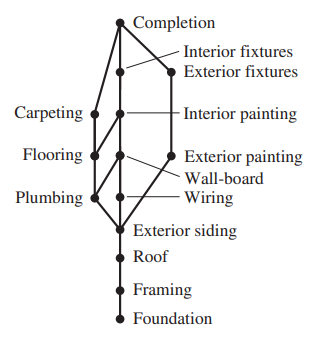
\includegraphics[]{images/HW12q66.PNG}
\end{center}
Foundation $\prec$ Framing $\prec$ Roof $\prec$ Exterior siding $\prec$ Wiring $\prec$ Plumbing $\prec$ Flooring $\prec$ Wall-board $\prec$ Exterior painting $\prec$ Interior painting $\prec$ Carpeting $\prec$ Interior fixtures $\prec$ Exterior fixtures $\prec$ Completion.

\end{document}
